\documentclass[beamer=true]{standalone}
\usepackage{../../preamblesnotes}

\begin{document}
\settitle{波動Wave motion}{波動學第一課 II}{周末班}

% longitudinal -> phase

\section{phase}
\begin{frame}
    \frametitle{相位Phase}

    \begin{itemize}
        \item 每個質點可以有不同的相位。\\Particles can have different phases.
        \item 兩個距離為 0$\lambda$、1$\lambda$、2$\lambda$、... 的質點屬於\textbf{同相}。
              \\Particles that are at distances of 0$\lambda$, 1$\lambda$, 2$\lambda$, ... are \textbf{same phase}.
        \item 兩個距離為 $\frac{1}{2}\lambda$、$1\frac{1}{2}\lambda$、$2\frac{1}{2}\lambda$、... 的質點屬於\textbf{反相}。\\Particles that are at distances of $\frac{1}{2}\lambda$, $1\frac{1}{2}\lambda$, $2\frac{1}{2}\lambda$, ... are \textbf{anti-phase}.
        \item 不是同相也不是反相的質點屬於\textbf{異相}。\\Particles that are neither in-phase nor anti-phase are \textbf{out-of-phase}.
    \end{itemize}
\end{frame}

\begin{frame}
    \frametitle{相位Phase}

    % \par{\par\centering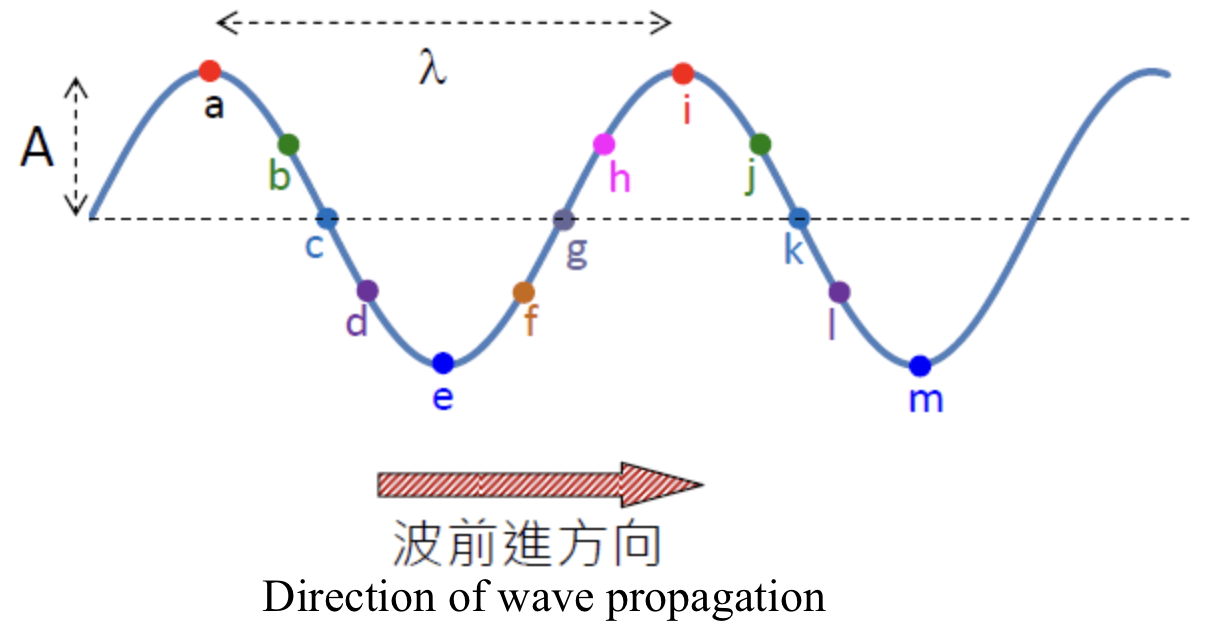
\includegraphics[width=.8\textwidth]{./img/ch1b_2024-05-17-14-08-57.png}\par}
    \par{\par\centering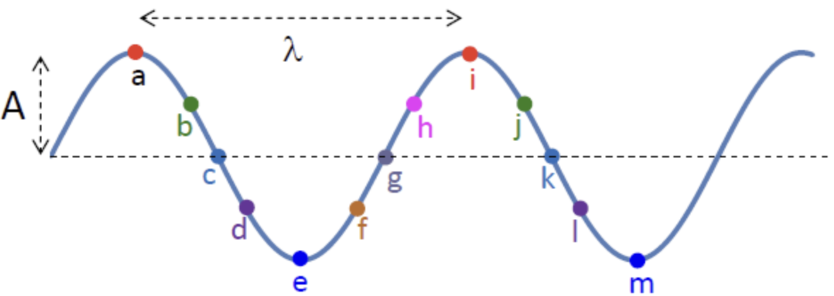
\includegraphics[width=\textwidth]{./img/ch1b_2024-05-17-14-18-34.png}\par}
    % 同相的粒子對:\hfill 反相的粒子對:\hfill 異相的粒子對:
    % \\in-phase pairs: \hfill anti-phase pairs: \hfill out of phase pairs:
    % \usepackage{longtable}


    \begin{longtable}{>{\hspace{0pt}}m{0.294\linewidth}|>{\hspace{0pt}}m{0.313\linewidth}|>{\hspace{0pt}}m{0.331\linewidth}}
        同相的粒子對\par{}in-phase pairs & 反相的粒子對\par{}anti-phase pairs & 異相的粒子對\par{}out of phase pairs  \endfirsthead
        \hline
                                   &                              &                                               \\
                                   &                              &                                               \\
                                   &                              &                                               \\
                                   &                              &                                               \\
    \end{longtable}

\end{frame}

\begin{frame}
    \frametitle{相位差phase difference}
    \begin{itemize}
        \item 同相的質點之間的距離為0$\lambda$、1$\lambda$、2$\lambda$、...,\\The distance between two in-phase particles is  0$\lambda$、1$\lambda$、2$\lambda$、...,\par 相位差分別為 The phase difference is respectively $0(=0^\circ)$、$2\pi(=360^\circ)$、$4\pi(=720^\circ)$、...
        \item 反相的質點之間的距離為$\frac{1}{2}\lambda$、$1\frac{1}{2}\lambda$、$2\frac{1}{2}\lambda$、... ,\\The distance between two anti-phase particles is $\frac{1}{2}\lambda$、$1\frac{1}{2}\lambda$、$2\frac{1}{2}\lambda$、... ,\par 相位差分別為$\pi(=180^\circ)$、$3\pi(=540^\circ)$、$5\pi(=900^\circ)$、...\\The phase difference is respectively $\pi(=180^\circ)$、$3\pi(=540^\circ)$、$5\pi(=900^\circ)$、...
    \end{itemize}


\end{frame}
\begin{frame}
    \frametitle{相位差phase difference}
    \begin{itemize}
        \item 同相的質點必定在任何時候以\textbf{相同}方向移動。\\Particles in phase must always move in the \textbf{same} direction at any given time.
        \item 反相的質點必定在任何時候以\textbf{相反}方向移動。\\Particles out of phase must always move in the \textbf{opposite} directions at any given time.
        \item 兩個同相(反相)的質點的速率可以是不一樣。\\The speeds of two particles in phase (out of phase) can be different.


    \end{itemize}


\end{frame}



\section{longitudinal}
% \begin{frame}
%     \frametitle{位置關係線圖 More about displacement relation graphs}
%     以下是
%     一列橫向行波在繩子上產生。下圖顯示位於$x$ = 0的粒子P的運動。在$t$ = 0時,位移為零而最接近$P$的粒子與$P$相距5 cm。
%     \par{\par\centering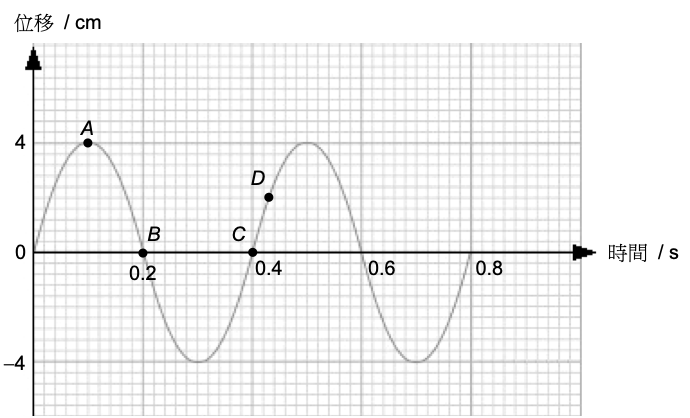
\includegraphics[width=.6\textwidth]{./img/ch1_earlyclass_wave_lq_2024-05-13-13-14-39.png}\par}
%     \begin{itemize}
%         \item [(a)] 解釋甚麼是橫波,並在上述的波以外舉一個例子。
%     \end{itemize}


% \end{frame}
% \begin{frame}[t]{例題Example}

% \end{frame}

\begin{frame}
    \frametitle{縱行波Longitudinal travelling wave}
    \par{\par\centering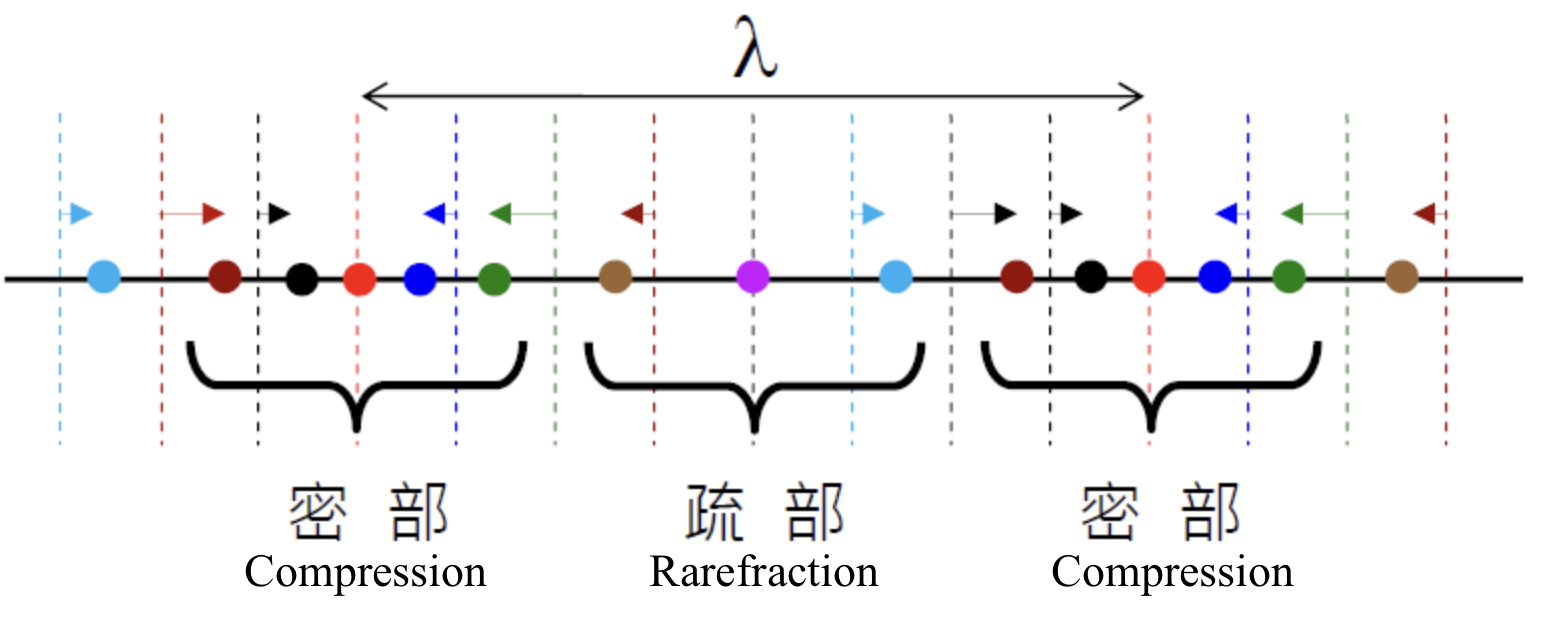
\includegraphics[width=\textwidth]{./img/ch1b_2024-05-17-13-51-46.png}\par}
    \begin{itemize}
        \item 上圖粒子上的箭矢是位移,不是速度。\\The arrows in the above diagram are displacements, not velocities.
    \end{itemize}
\end{frame}



\begin{frame}
    \frametitle{以位移距離線圖來表達縱波Representing Longitudinal Waves on Displacement-distance graph}

    \par{\par\centering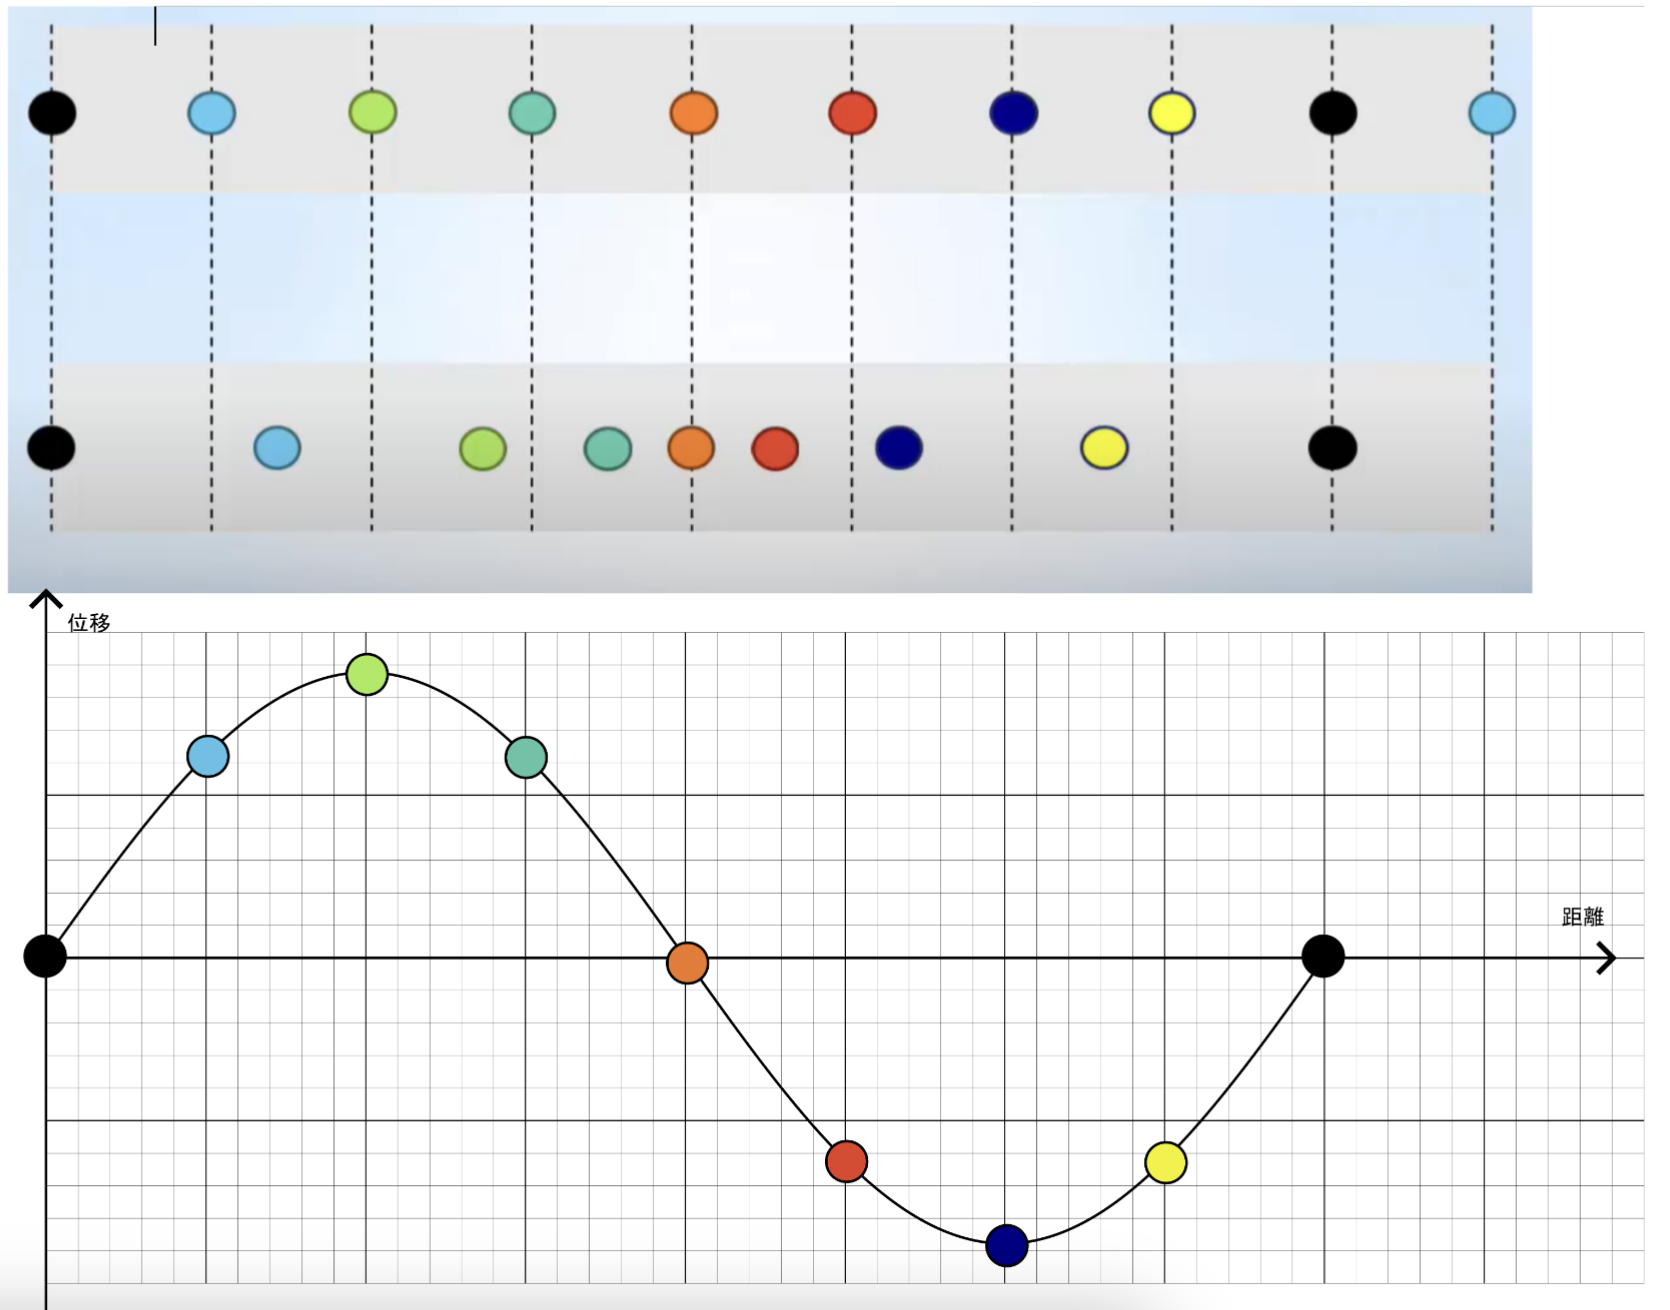
\includegraphics[width=.8\textwidth]{./img/ch1b_2024-05-17-12-14-25.png}\par}

\end{frame}


\begin{frame}
    \frametitle{以位移距離線圖來表達縱波Representing Longitudinal Waves on Displacement-distance graph}

    \par{\par\centering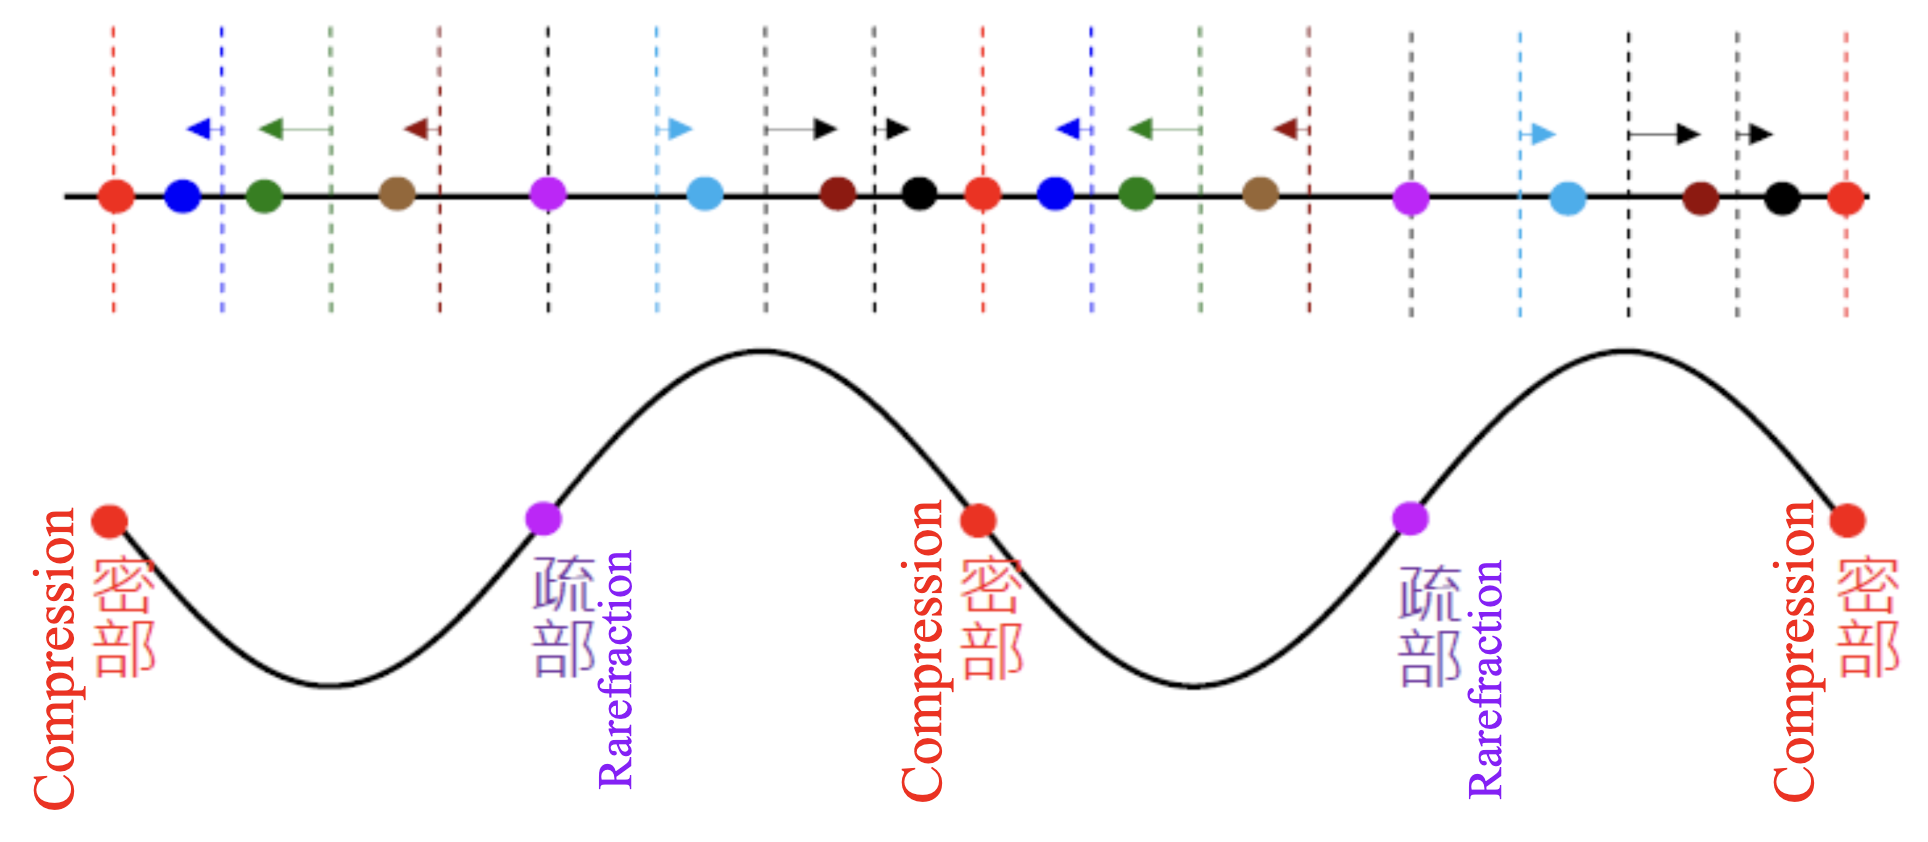
\includegraphics[width=\textwidth]{./img/ch1_2024-05-16-13-49-44.png}\par}

\end{frame}

\begin{frame}
    \frametitle{以位移距離線圖來表達縱波Representing Longitudinal Waves on Displacement-distance graph}
    \par{\par\centering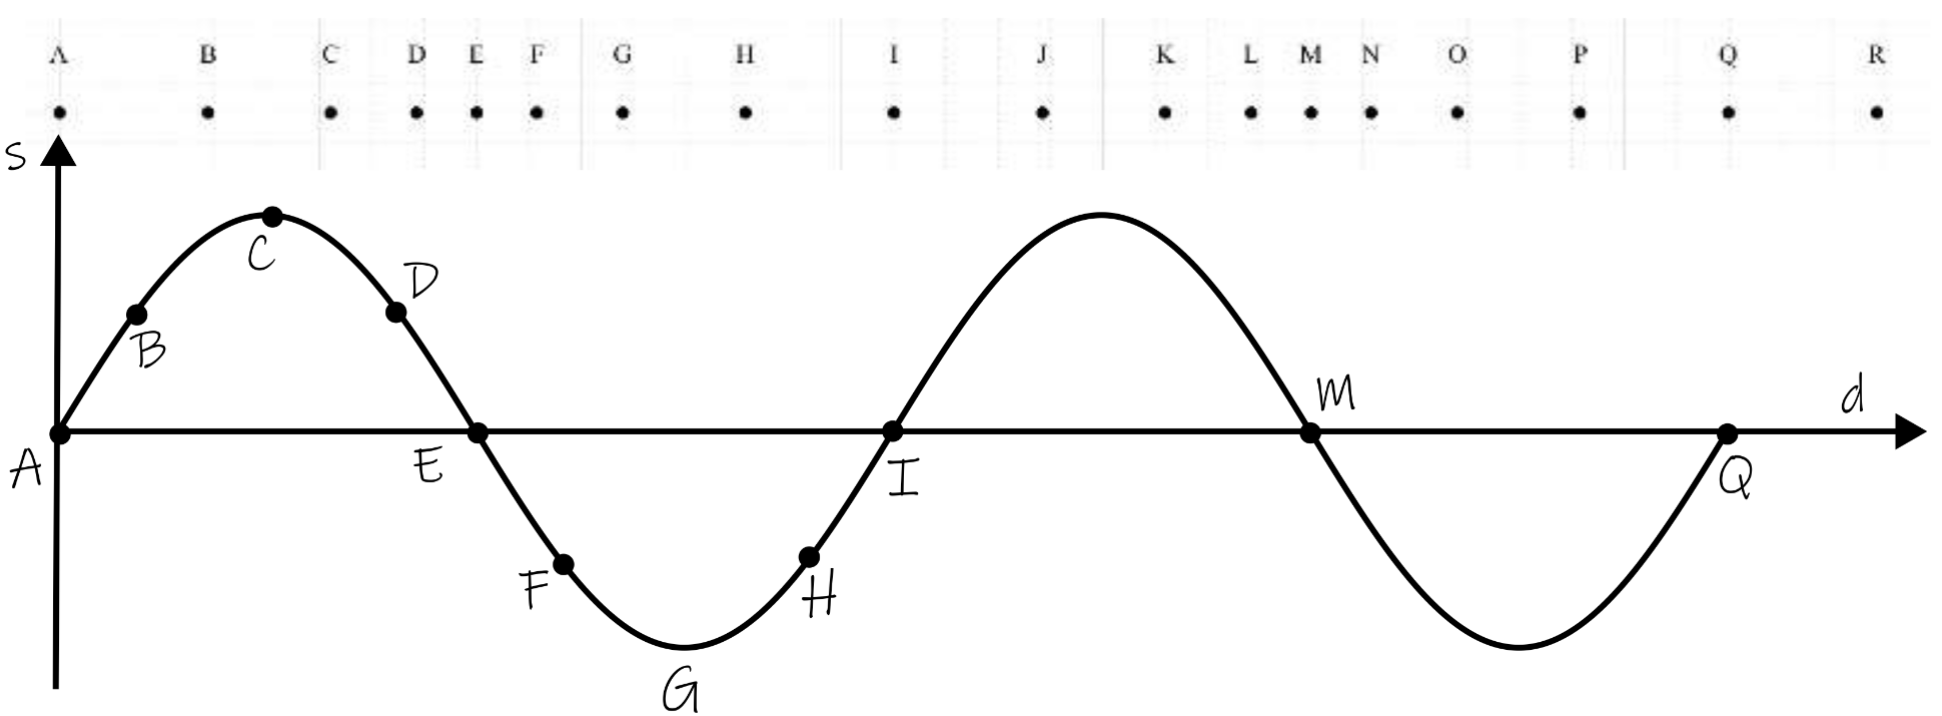
\includegraphics[width=\textwidth]{./img/ch1b_2024-05-17-12-15-17.png}\par}
\end{frame}

% \begin{frame}[t]
%     \frametitle{}

%     \par{\par\centering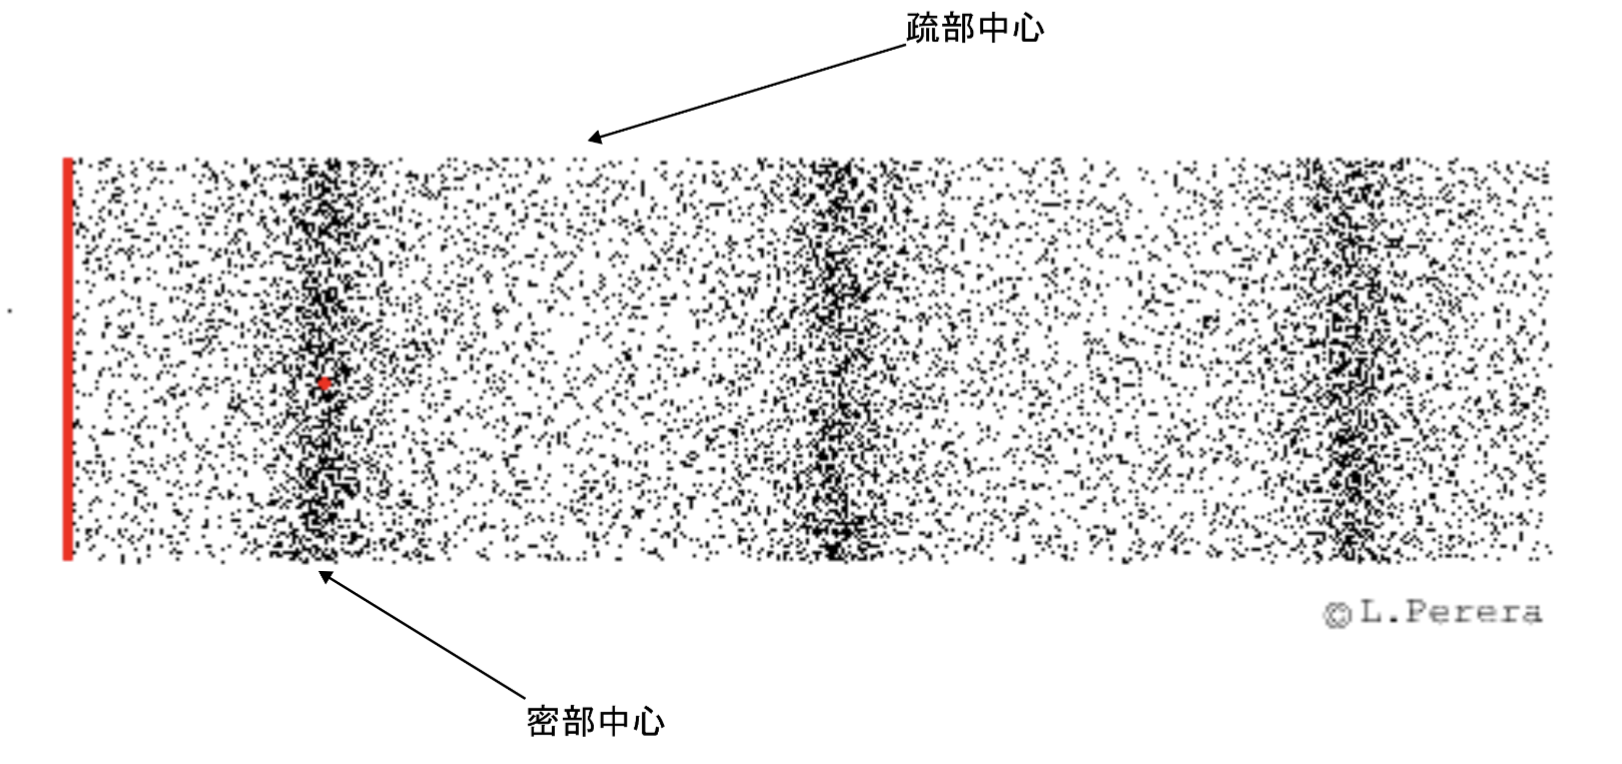
\includegraphics[width=\textwidth]{./img/ch1b_2024-05-17-12-16-03.png}\par}

% \end{frame}

\begin{frame}
    \frametitle{縱行波Longitudinal travelling wave}

    \begin{itemize}
        \item \textbf{密/疏部中心} $\Leftrightarrow$ 其粒子位於\textbf{平衡位置}\\\textbf{Centers of compressions / rarefactions} $\Leftrightarrow$  particles at \textbf{equilibrium position}
        \item 縱波的密部 / 疏部的中央\textbf{並不對應}於橫波的 波峰 / 波谷。\\Centers of compressions / rarefactions of a longitudinal traveling wave are \textbf{NOT} the counterparts of the crests/ troughs of a transverse traveling wave.
        \item 密部內所有粒子的速度方向均與縱波傳播的方向相同 。 反之,疏部內所有粒子的速度方向與縱波傳播的方向相反。\\All particles inside a compression are moving in the same direction of the propagation of the wave, while those inside a rarefaction are moving in the opposite direction.
        \item 密部和疏部的中央,位移是零但速率均是最大。\\At the central part of a compression or a rarefaction, the displacement is zero and the speed is the greatest.
    \end{itemize}
\end{frame}

\begin{frame}[t]{例題Example}
    \par{\par\centering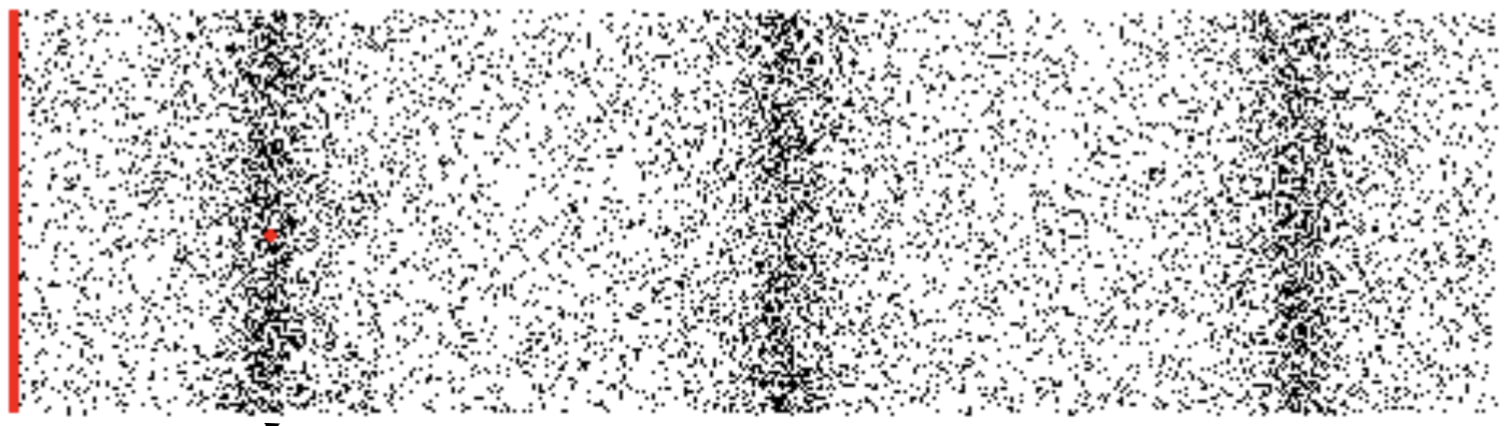
\includegraphics[width=\textwidth]{./img/ch1b_2024-05-17-12-16-45.png}\par}
\end{frame}

\begin{frame}[t]{例題Example}
    \par{\par\centering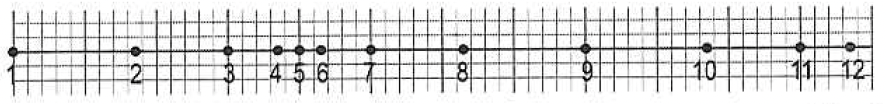
\includegraphics[width=\textwidth]{./img/ch1b_2024-05-17-12-41-10.png}\par}
    上面的圖示顯示了在某一瞬間,一個聲波從左向右傳播時,空氣粒子的位置。\\The above figure shows the positions of the air particles when a sound wave is travelling from left to right at a certain instant.
    \vfill\raggedleft Next page...
\end{frame}

\begin{frame}[t]{例題Example}
    以下關於聲波中密部中心位置的敘述哪些是正確的?\\Which of the following statements about the position of the centre of compression in the sound wave are correct?
    \begin{statements}
        \task 位置5的粒子位於密部中心。\\Particle at position 5 is at the centre of compression.
        \task 靠近密部中心的兩側粒子正在朝向其移動。\\Particles on both sides immediately next to the centre of compression are moving towards it.
        \task 在聲波中,密部中心處的氣壓最高。\\The air pressure is the highest at the centre of compression in the sound wave.
    \end{statements}
    \vfill\raggedleft Next page...
\end{frame}

\begin{frame}[t]{例題Example}
    (承上題)關於在圖中所示的聲波中的粒子5,以下哪些敘述是正確的?\\Which of the following statements about particle 5 in the sound wave at the instant shown in the figure are correct?
    \begin{statements}
        \task 它的位移為零。\\Its displacement is zero.
        \task 與波中的其他空氣分子相比,它的速度是最大的。\\Its velocity is the largest compared to other air molecules in the wave.
        \task 與波中的其他空氣分子相比,它的加速度是最大的。\\Its acceleration is the largest compared to other air molecules in the wave.
    \end{statements}
    \vfill\raggedleft Next page...
\end{frame}

\begin{frame}[t]{例題Example}
    (承上上題)以下哪對粒子是同相振動的?\\Which of the following pairs of particles are vibrating in phase?
    \begin{statements}
        \task 位於位置1和位置5的粒子。\\Particles at positions 1 and 5
        \task 位於位置1和位置9的粒子。\\Particles at positions 1 and 9
        \task 位於位置9和位置11的粒子。Particles at positions 3 and 11
    \end{statements}

    \vfill\raggedleft Next page...
\end{frame}

\begin{frame}[t]{例題Example}
    (承上上上題)在所示瞬間之後,位置1和7的粒子運動方向如何?\\What are the directions of motion of particles at positions 1 and 7 immediately after the instant shown?
    \begin{tasks}
        \task [] \textbf{1} \dtab \textbf{7}
        \task $\rightarrow $ \dtab 瞬時靜止Momentarily at rest
        \task $\leftarrow $ \dtab 瞬時靜止Momentarily at rest
        \task $\leftarrow $ \dtab $\rightarrow $
        \task $\rightarrow $ \dtab $\leftarrow $
    \end{tasks}
    \vfill\raggedleft Completed.
\end{frame}



\begin{frame}[t]{例題Example}
    % aristo p7

    下圖展示了一個縱波在某一瞬間從左向右傳播。\\The following diagram shows a longitudinal wave travelling from left to right at a certain instant.
    \par{\par\centering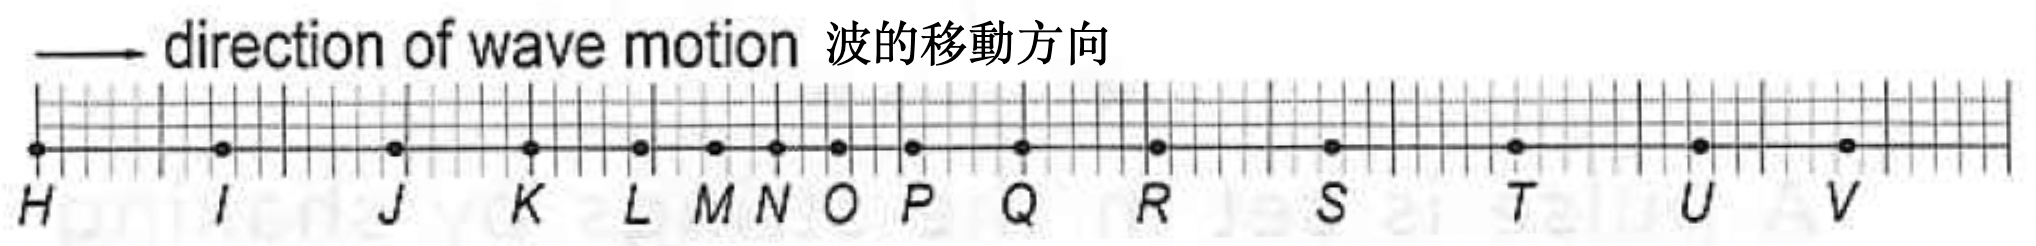
\includegraphics[width=.9\textwidth]{./img/ch1b_2024-05-17-12-25-33.png}\par}
    \raggedleft Next page...
\end{frame}

\begin{frame}[t]{例題Example}
    下列哪項陳述是正確的?\\Which of the following statements is correct?
    \begin{tasks}
        \task 在H和V之間的距離是$1.5\lambda$。\\The distance between H and V is $1.5\lambda$.
        \task 位置K的粒子達到了最大位移。\\The particle at position K is at its maximum displacement.
        \task 在所示瞬間,位於位置R的粒子向右移動。\\The particle at position R is moving to the riaht at the instant shown.
        \task 位於位置M和位置S的粒子在同相振動。\\Particles at positions M and S are vibrating in phase.
    \end{tasks}
    \raggedleft Next page...
\end{frame}


\begin{frame}[t]{例題Example}
    \par{\par\centering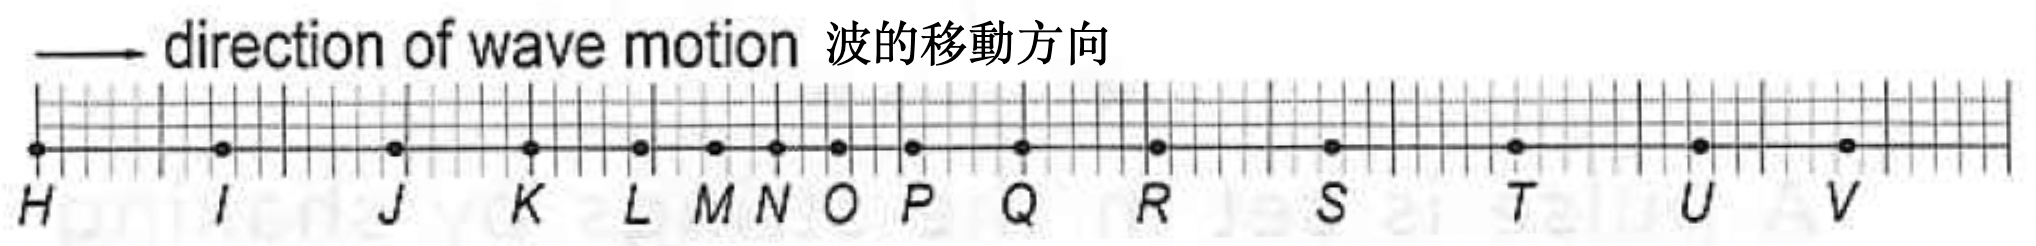
\includegraphics[width=.9\textwidth]{./img/ch1b_2024-05-17-12-25-33.png}\par}
    (承上題)相對於位置$H$的粒子,以下哪個粒子的振動相位相差 \dg{180}?\\Which of the following particles is vibrating \dg{180} out of phase relative to particle at position $H$?
    \begin{tasks}
        \task $J$
        \task $L$
        \task $N$
        \task $P$
    \end{tasks}
    \vfill\raggedleft Completed.
\end{frame}

































































































\end{document}